\chapter{Implementation}
A requirement of mine for the software environment was that it allows me to easily debug and implement changes, and that there is a significant support for the chosen language and frameworks. Personal preferences in style have also weighted in.
 
\section{Software environment}
I have chosen Python as the programming language for the implementation. A compelling argument is that it has more or less become the language of machine learning, especially for programmers; with lots of libraries and packages available, as well as online tutorials. It also allows for very laconic expressions, which suits me well. A compelling counter argument for why this is not an optimal language for deep learning, and especially in this project where computational power is limited in comparison to what I am trying to mimic, is that Python is an interpreted language. This makes running it significantly slower, compared to a compilable language like C. However, this problem is partially mitigatable, which I will touch on later.

Among stand-alone deep learning frameworks for Python there exists two mastodons: Tensorflow and PyTorch. The first is actively developed by Google, the other by Facebook\cite{Hale2019}. Tensorflow has been longer in the game, and might have a larger traction. PyTorch on the other hand offers a more python-esque way of writing code, and has a dynamic computational graph, which allows for loops and conditional code inside the network model. PyTorch has also been shown, in some tests, to be able to perform both forward and backward propagation faster than Tensorflow\cite{John2018}. As a result I chose PyTorch as the deep learning framework to be used in the implementation.

\section{Implementation strategy}
In order to be able to answer the question from the problem definition in a scientific manner, I need to test how various configurations and parameter tweakings change the relationship between learned skill and the required computational effort.

I have decided that a game complexity of the size of Go on a 19x19 board would be too ambitious. It would still, however, be interesting to investigate how changing the complexity of the game being played affects the learned skill and needed processing power, measured by running time. I have settled on training agent models on board shapes 7x7 and 9x9.

To safely test the various configuration of the algorithm, the code contains a \textit{config} object. This is created when the algorithm is started, and is used extensively when the algorithm runs. Having algorithm parameters and boolean control variables gathered at one place, made it easy to keep track of changes. Several of the variables can be set directly from the terminal, when starting training of an agent model. Doing it this way, I avoided having to directly change the code for some part, if I wanted to test something else. For instance, in the implementation of the network, a variable is consulted in whether forward propagation should be following the original residual block design\footnote{See figure \ref{fig-res-block}.} or full pre-activation \footnote{See figure \ref{fig-fpa-block}.}.

\section{Optimization}
To generate enough trained agents, and play them against each other, inside the time scope of this project, an optimized code base was needed. As mentioned earlier, Python is an interpreted language which affects how fast it runs. Additionally, Python, as implemented by CPython, is not really suited for multi-threading, as it employs what is know as the Global Interpreter Lock (GIL)\cite{GlobalInterpreterLock2017}.

\subsection{Numba}
To get around the slowness in Python, resulting from the fact that it is interpreted, I use the just-in-time compiler \textit{numba}. Numba translates part of the code into machine code, which enables it to run much faster. To actually gain a performance boost from this, it should not be used on Python objects, as the GIL will then hamper execution speed. However, both regular primitive values, and most python and numpy collections, of fixed length, can be utilized. Numba especially improves performance of code that run loops.

\subsection{Playing and training in batches}
I decided against trying to parallelize the code running on the CPU with either threads or multiprocessing, because of the GIL. Instead, to improve the running performance, I made use of PyTorch built-in functionality to make neural networks work on batches of data, thus utilizing parallel data processing on the GPU. This improved the running performance of the algorithm tremendously, allowing self-play game data to be generated in less time, and training on said data much faster.

\subsection{Half-precision}
A final optimization that was done was to use half-precision floating points. As touched on previously, the Nvidia RTX GPUs contains Tensor cores. To use these, the data needs to be half-precision. Initially I tried doing the neural networks and all input in half-precision, but at some point I experienced a network where all the weights of a particular network ended up being $\textit{NaN}$. Without being completely certain, this probably happened because some accumulator value became too large to represent in binary16, thus becoming $\infty$, spread this value to other variables, and finally ended up with diving two infinite numbers, resulting in $\textit{NaN}$.

The final code contains the option to use mixed precision and single precision. With mixed precision, a single precision master version of the network is kept at all time. It is this model that is trained, on single precision input. I did not feel confident enough to attempt the exact same mixed-precision training techniques described by \citeauthor{Micikevicius2018}: weight scaling to avoid vanishing gradients, and only converting accumulators to single precision\cite{Micikevicius2018}. However, under my version of mixed precision, all self-play games are played with a copy of the network, where all network layers, except for Batch Normalization which does accumulation, are converted to half-precision.

A last place where single precision is used, and at all times, is when saving algorithm data to disk. Here all game data is converted to numpy's implemenation of the binary16 datatype, float16. Before I did this, game data values were saved as regular Python floats, which are objects that take up 64 bits each. The result being that disk space used by game data was reduced by a factor of $\approx 4$.

\section{Hex}
The game of Hex was implemented in the simplest possible way. It contains several functions that are used by the algorithm: \textit{initial\_state(size)}, \textit{actions(state)}, \textit{player(state)}, \textit{utility(state, player)}, \textit{terminal\_test(state)}, and \textit{result(state, action)}. The functions return exactly what their names imply.

As can be seen, at the core of all these functions is a \textit{state}. A state has been modelled as a class with information relevant to these functions. Among the most important variables is the board, conceptualized as a 2-dimensional board\footnote{But in the code actually modelled as a 1-dimensional list.}, where $0$ represents an unoccupied board position, $1$ occupied by the first player, and $-1$ is occupied by the second player. Using a conceptually 2D board as a hexagonal grid is possible when certain restrictions are applied on the possible directions of connection. An illustration of this can be seen in figure \ref{fig-2d-hex}.

\begin{figure}[ht]
	\centering
	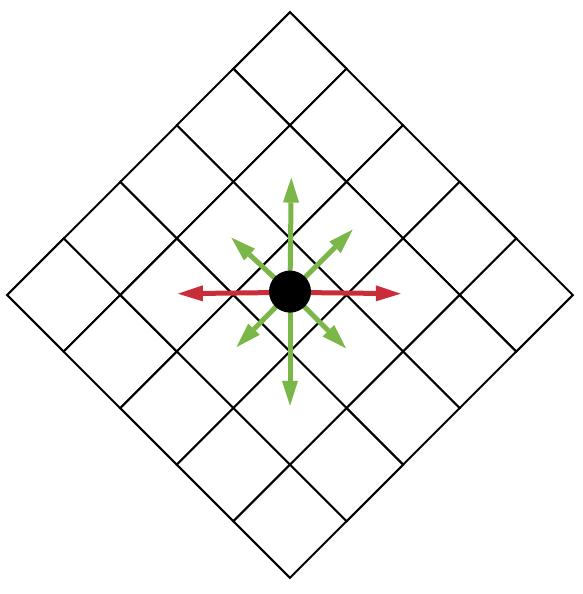
\includegraphics[width=0.35\textwidth]{figures/2d-to-hex}
	\caption{Example of using a 2D array as a hexagonal grid representation, by only allowing connections between the cells with a green line, and disallowing the ones marked with a red line. The result is that only 6 connections are possible, making the board practically hexagonal.}
	\label{fig-2d-hex}
\end{figure}

A state also includes a list of actions taken previously, in the form an list of integers is kept, for quickly creating input images for the neural network. Available actions are stored as a set, to quickly remove an element when an action is taken. Finally it also includes an array used in the Quick-Find variant of the Union-Find algorithm by \citeauthor{Sedgewick2011}\cite{Sedgewick2011}. This is used to quickly determine if a game state is terminal, i.e. a player has connected its two sides. This array contains an entry for each positions on the board, and also 4 entries representing the sides of the board. That way it is easy to keep track of what is connected, in regards to the rules of Hex.

To further minimize the computational footprint of the game implementation, almost all functions are fully or partially compiled by numba during run time. The result is that the game itself is the least concern in regards to the running performance of the algorithm.

\section{The learning agent algorithm}
The algorithm has been implemented according to the outline presented in figure \ref{fig-az-algorithm}. In the following I will delve a bit more into the details. What is not seen in that figure, is that in my implementation games are played in batches of 50. Furthermore, between each batch run of self-play games, the network trains for 10 iterations. What was needed to be balanced was processing speed, but also getting sufficient data for the algorithm, and for the network, not to train too much or train too little. The latter is important early on when the agent who played the games are not very smart, and we want to avoid overfitting. The numbers 50 and 10 were found after trying different sizes of varying success, with these showing good results, when I examined their training loss rates.

Because of the limitation on processing power the number of MCTS simulations was set to 200. This value was kept for both on 7x7 and 9x9 boards. AlphaZero used 800 simulations for all its games. For Go on a 19x19 board, that amounted to a mean of $\approx 2.22$ visits for each child node of the initial state. For Hex, on 7x7 and 9x9 boards, it amounts to $\approx 4.08$ and $\approx 2.47$ respectively. I found it to be a reasonable sample sizes, when keeping in mind what AlphaZero employed for Go with its larger complexity.

\begin{equation}
UCB(p,c) = \frac{V_c}{N_c} + 1.27\times P_c\times \sqrt{\frac{N_p}{1 + N_c}}
\label{eq-ucb-formula}
\end{equation}

The balance between exploration and exploitation, in the MCTS part of my algorithm, is done by the version of UCB seen in equation \ref{eq-ucb-formula}. This is very similar to equation \ref{puct-2} and \ref{puct-3} from the previous chapter, with the only difference that $C(p)$ has been replaced by an exploration constant of $1.27$. Had this constant been higher, more states would have been visited, potentially helping avoid a horizon effect, but at the cost of being less certain about the most promising actions. When the maximum number of MCTS simulations has been reached, and an action selection is performed by doing ArgMax on the root's child nodes' visit counts.

\subsection{Mitigating horizon effect}
The probabilistic random selection of actions, mentioned earlier, has also been implemented for an initial number of steps during each training game. This is set to a game's maximum length divided by 10, and ceiled. For a 7x7 board it means that this form of selection is active for the first 5 moves of the game, and for 9x9 the first 9. The probabilistic values are created with values fed to a Softmax function. The values are the normalized visit counts for the root's child nodes. The normalization is to avoid less frequently visited nodes gaining a probability of practically zero, if the distribution is very skewed. Having all the values be below 1 flattens the distribution curve, elevates the less visited nodes' probability, and lowers that of the most visited. To prevent it becoming too flat, all values are multiplied by $1.5$ before Softmax. 

Dirichlet noise is also being added to the prior values, with the network's prior predictions counting for $3/4$, and the normalized dirichlet values counting for $1/4$. In the config object, the dirichlet $\alpha$-value is set to $10$ divided by the average number of legal moves of the game. This I have estimated, for Hex, to be the number of board positions multiplied by $0.7$. In retrospect, this estimation is put way too high, especially for games where the playing agents know what they are doing. But from experience, the number seemed to work fine in creating suitable $\alpha$-values, and was automatically adjusted when the board dimensions were changed. Sorted examples of how the noise distributions can look, after they have been normalized and multiplied a factor of 0.25, can be seen in figure \ref{fig-dir-dist}.

\begin{figure}[ht]
	\centering
	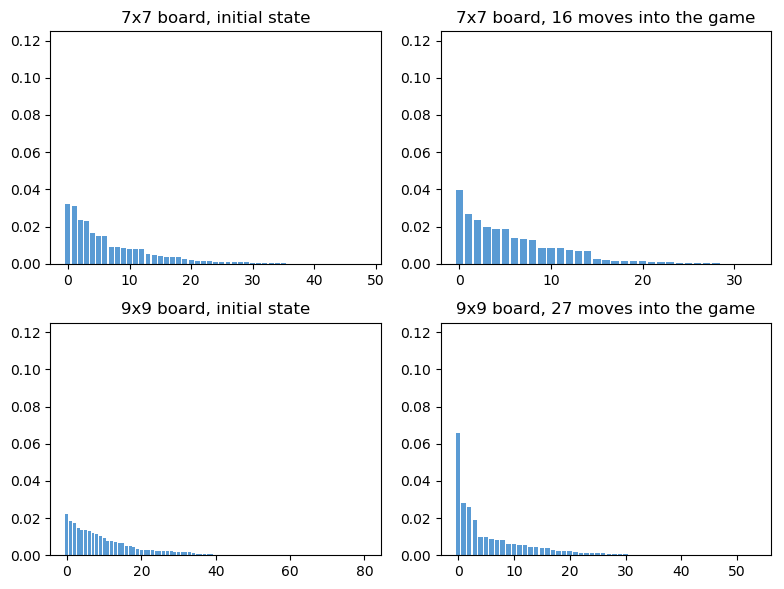
\includegraphics[width=0.8\textwidth]{figures/dirichlet-dist}
	\caption{Example of 4 different sorted dirichlet noise distributions, after values have been normalized to a sum of 1, and then multiplied by a factor 0.25.}
	\label{fig-dir-dist}
\end{figure}

\subsection{Network structure}
The neural network is set to build residual blocks with convolutional layers of channels size 256 and stride 1. Earlier attempts at setting the number of channels to 128 greatly improved speed, and the networks size on disk, but it hampered accuracy enough for me to raise it. The network can have its number of residual blocks adjusted. I ended up testing residual block counts of 13 and 19, to see how much impact it has having it lower than AlphaZero's 19. Furthermore, it can also be tasked with doing forward propagation either in accordance with the original residual block design\footnote{See figure \ref{fig-res-block} for an illustration.} or the full pre-activation design\footnote{See figure \ref{fig-fpa-block} for an illustration.}\cite{HeKaimingandZhangXiangyuandRenShaoqingandSun2016, He2016}. Otherwise it is built pretty much as described by \citeauthor{Silver2018}, and shown in figure \ref{fig-network-structure}. 

\subsection{Training}
Training is done with a Stochastic Gradient Descent optimizer that uses a momentum\footnote{A technique used to speed up Gradient Descent convergence.} of $0.9$ , weight decay\footnote{Used for regularization of weights, to prevent overfitting} of $0.0001$, and a learning rate of $0.05$. The first two are similar to the ones used by AlphaZero, but the last is 4 times lower. This was found by brute forcing, as my implementation resulted in loss rates that would be all over the place when it was higher. Unlike AlphaZero the learning rate is not lowered as the algorithm progresses for several numbers of games being played.

The loss functions are Mean Squared Error for values, seen in equation \ref{eq-mse}, and Softmax Cross-Entropy with Logits for policies, seen in equation \ref{eq-softmax-cross-entropy}. For equation \ref{eq-softmax-cross-entropy} the multiplication in $Log(Softmax(\hat{Y_i})) \times Y_i$ is an element-wise multiplication, not a matrix multiplication.

\begin{equation}
MSE = \frac{1}{n} \times \sum_{i = 1}^{n} \left(Y_i - \hat{Y_i}\right)^2
\label{eq-mse}
\end{equation}

\begin{equation}
SoftmaxCrossEntropyLogits = \frac{1}{n} \times -\sum_{i = 1}^{n} \left( Log(Softmax(\hat{Y_i})) \times Y_i\right)
\label{eq-softmax-cross-entropy}
\end{equation}

\subsection{Network input}
Providing the network information about a board state is, everything considered, domain-specific knowledge. However, I have strived to make the features included as minimal as possible. 

Input is provided to the network as images of features, in the form of PyTorch tensors\footnote{A PyTorch tensor is basically a matrix array.}. For a 9x9 board it has the shape of $batch size \times 2  \times 9 \times 9$. Here the number 2 is the amount of channels. I have reserved the first channel for a binary representation of where the player whose turn it is, has pieces on the board. The other channel is for the opponent's pieces. 

As such, the features given to the network is very minimal. It is not given information about how connection restrictions are applied to use the 2D board array as a hexagonal grid, and it is not given information about which realized connections exist for either player. These elements is up to the networks to learn themselves.

One trick on the input, to ease the learning, is applied. That is, if it is the second player's turn, both channel board images are transposed, such that the perspective emulate that of the first player, in terms of the turn taking player's goal sides, and which belongs to the opponent.

\subsection{Other parameters}
For each 5 of the play-50-games-train-network-10-times iterations, everything of interest is saved to disk. This includes the network, the config object, the 1,000 or 500 most recent games, the loss values recorded during training, the time spent running, etc.. This makes it possible to stop the algorithm, for whatever reason, and restarting it again from the last save, or use it for normal play mode.
